% ------------------------------------------------------------------------------
% LaTeX Template: Presentation Slides
% This is LaTeX template is suitable for (technical) presentations
%
% Copyright: Marius Hofert, Markus Kohm (PracTeX)
% The idea of this template came from The PracTeX Journal 2010-2
% Date: April 2011
% ------------------------------------------------------------------------------

% ------------------------------------------------------------------------------
% Document
% ------------------------------------------------------------------------------
\documentclass[
	paper=128mm:96mm,	% like beamer
	fontsize=11pt,					% like beamer
	pagesize,							% write page size to dvi or pdf
	parskip=half-,					% paragraphs separated half a line, no marking of line endings
	numbers=noendperiod,	% removes points for special parts (e.g. appendix)
	captions=nooneline			% do not distinguish between one or more lines in captions
	]{scrartcl}							% KOMA script (article)

% Presentation tweaks	
\linespread{1.12} 				% enlarge line space

% Color
\usepackage{xcolor}			% color package; load before tocstyle

% Page structure
\usepackage{calc}				% working with lengths, counters etc.
\usepackage[
	includeheadfoot,%
	top=3.5mm,%
	bottom=3.5mm,%
	left=5.5mm,%
	right=5.5mm,%
	headsep=6.5mm,%
	footskip=8.5mm%
	]{geometry}						% set page layout parameters
\usepackage{scrpage2}		% package for page style with not only uppercase letters in the head 
\usepackage{titlesec}			% for reducing space between ((sub)sub)sections and text
\usepackage{tocstyle}			% for adjusting table of contents

% ------------------------------------------------------------------------------
% Document metadata
% Fill in your own stuff here
% ------------------------------------------------------------------------------
\newcommand*{\mytitle}{Watermark Road Maps against Crop and Merge Attacks}		% title
\newcommand*{\mytitleontitlepage}{\mytitle}	% title
\newcommand*{\runninghead}{Watermark Road Maps against Crop and Merge Attacks} % Running head displayed on almost all slides
\newcommand*{\myauthor}{Jacky Jiang, Kenny Zhu, Yan Huang and Xiaobin Ma}				% name
\newcommand*{\abbrauthor}{Jacky Jiang, et al.}				% name
\newcommand*{\mydate}{June 19, 2013}						% date
\newcommand*{\myuni}{\url{adapt.seiee.sjtu.edu.cn}}			% university/department

% colors
\definecolor{mygreen}{RGB}{44,85,17}				% for emphasizing text (#2c5511)
\definecolor{myblue}{RGB}{34,31,217}					% for emphasizing text (#5d90c2)
\definecolor{mybrown}{RGB}{194,164,113}			% for emphasizing text (#c2a471)
\definecolor{myred}{RGB}{255,66,56}					% for emphasizing text (#cc7b76)
\newcommand*{\mygreen}[1]{\textcolor{mygreen}{#1}}
\newcommand*{\myblue}[1]{\textcolor{myblue}{#1}}
\newcommand*{\mybrown}[1]{\textcolor{mybrown}{#1}}
\newcommand*{\myred}[1]{\textcolor{myred}{#1}}

% ------------------------------------------------------------------------------
% Fonts
% ------------------------------------------------------------------------------
\usepackage[T1]{fontenc}	% for correct hyphenation and T1 encoding
\usepackage{bookman}			% latin modern font

% Choose one of the following three fonts
%\usepackage{fourier}			% utopia
\usepackage{charter}			% low-resolution roman font
%\renewcommand{\familydefault}{\sfdefault}% sans serif

\usepackage[english]{babel}% for Brittish English
\usepackage{microtype}		% for character protrusion and font expansion (only with pdflatex)

% ------------------------------------------------------------------------------
% Misc
% ------------------------------------------------------------------------------ 
\usepackage{amsthm}			% theorem environments
\usepackage{bm}					% for bold math symbols
\usepackage{enumitem}		% for automatic numbering of new enumerate environments
\usepackage{graphicx}		% for including figures
\usepackage{epsfig}
\usepackage{subfigure}
\usepackage[noend]{algpseudocode}
\usepackage{tikz}				% sophisticated graphics package
\usepackage{tabularx}			% for special table environment (tabularx-table)
\usepackage{booktabs}		% for table layout
\usepackage[
	hypertexnames=false,		% for correct links (duplicate-error solution)
	setpagesize=false,			% to prevent change text-/paperformat for the document
	pdfborder={0 0 0},			% removes border around links
	pdfpagemode=FullScreen,% open pdf in full screen mode
   pdfstartview=Fit				% fit page to pdf viewer
]{hyperref}							% all links stay black and are thus invisible
\hypersetup{						% NOTE: If \myauthor or \mytitle contain non-us-ascii-chars you
           									% should not use them inside \hyperref.
  pdfauthor=\myauthor,%
  pdftitle=\mytitle%
}
\usepackage{lastpage}			% to denote last page in slide numbering
\newcommand{\I}{\mathcal{I}}
\newcommand{\LEN}{\mathcal{L}}
\newcommand{\R}{\mathcal{R}}
\newcommand{\T}{\mathcal{T}}
\newcommand{\D}{\mathcal{D}}
\newcommand{\M}{\mathcal{M}}
% ------------------------------------------------------------------------------
% Page Style
% ------------------------------------------------------------------------------
\pagestyle{scrheadings}		% activates pagestyle from scrpage2
\clearscrheadfoot					% clear head and foot of scrheadings and scrplain
\setkomafont{pageheadfoot}{\normalfont\color{black}\sffamily}% setting for page head and foot

% optical vertical centering of page contents
\makeatletter
\renewcommand*{\@textbottom}{\vskip \z@ \@plus 1fil}
\newcommand*{\@texttop}{\vskip \z@ \@plus .5fil}
\addtolength{\parskip}{\z@\@plus .25fil}% stetch parskip a lot
\makeatother

% spacings
\titlespacing{\section}{0mm}{0mm}{0mm}% space (left, before, after) between section and text
\titlespacing{\subsection}{0mm}{0mm}{-1mm}% space (left, before, after) between subsection and text
\titlespacing{\subsubsection}{0mm}{0mm}{-2mm}% space (left, before, after) between subsubsection and text
\setcounter{secnumdepth}{2}% add numbering down to subsection 
%------------------------------------------------
% Header configuration - if you don't want a header remove this block
\ihead{
\hspace{-2mm}
\begin{tikzpicture}[remember picture,overlay]
\node [xshift=\paperwidth/2,yshift=-\headheight] (mybar) at (current page.north west)[rectangle,fill,inner sep=0pt,minimum width=\paperwidth,minimum height=2\headheight,top color=mygreen!64,bottom color=mygreen]{}; % Colored bar
\node[below of=mybar,yshift=3.3mm,rectangle,shade,inner sep=0pt,minimum width=128mm,minimum height =1.5mm,top color=black!50,bottom color=white]{}; % Shadow under the colored bar
shadow
\end{tikzpicture}
\color{white}\runninghead} % Header text defined by the \runninghead command below and colored white for contrast
%------------------------------------------------


% foot
\newlength{\footheight}
\setlength{\footheight}{8mm}
\addtokomafont{pagefoot}{\footnotesize}% general setting for the foot
\setkomafont{pagenumber}{\color{black}}% setting for page foot
\ifoot{% foot left
	\hspace{-2mm}%
	\begin{tikzpicture}[remember picture,overlay]
		\node [xshift=\paperwidth/2,yshift=\footheight] at (current page.south west)[rectangle,fill,inner sep=0pt,minimum width=\paperwidth,minimum height=3pt,top color=mygreen,bottom color=mygreen]{};% bar 
	\end{tikzpicture}%
	\abbrauthor\ \raisebox{0.2mm}{$\bm{\vert}$}\ \myuni
}
\ofoot[\pagemark/\pageref{LastPage}\hspace{-2mm}]{% foot right
	\pagemark/\pageref{LastPage}\hspace{-2mm}}

% table of contents
\AtBeginDocument{\renewcaptionname{english}{\contentsname}{\large Outline}}% change name of toc
\makeatletter
\newtocstyle[noonewithdot]{nodotnopagenumber}{% define tocstyle without dots and page numbers
  \settocfeature{pagenumberbox}{\@gobble}%
}
\makeatother
\usetocstyle{nodotnopagenumber}

% theorems
\newtheoremstyle{mythmstyle}%
	{0.5em}% space above
	{0.5em}% space below
	{}% body font
	{}% indent amount
	{\sffamily\bfseries}% head font
	{}% punctuation after head
	{\newline}% space after head
	{\thmname{#1}\ \thmnote{(#3)}}% head spec
\theoremstyle{mythmstyle}
\newtheorem{theorem}{Theorem}[section]
\newtheorem{remark}[theorem]{Remark}
\newtheorem{algorithm}[theorem]{Algorithm}
\renewcommand*\proofname{Proof}
\makeatletter% correct qed adjustment

% box 
\newcommand*{\mybox}[2]{% width, content
	\par\noindent
	\begin{tikzpicture}[
		mynodestyle/.style={rectangle,draw=mygreen,
											 thick,inner sep=2mm,text justified,top color=white,
											 bottom color=white,above}]%
		\node[mynodestyle,at={(0.5*#1+2mm+0.4pt,0)}]{%
			\begin{minipage}[t]{#1}
				#2
			\end{minipage}%
		};
	\end{tikzpicture}%	
	\par\vspace{-1.3em}
}


% ------------------------------------------------------------------------------
% Begin document
% ------------------------------------------------------------------------------
\begin{document}
%
% SLIDE1 ----------------------------------------------------------
%
\thispagestyle{empty}
% background (stroke)
\begin{tikzpicture}[remember picture,overlay]
	\node [xshift=\paperwidth/2,yshift=\paperheight/2] at (current page.south west)[rectangle,fill,inner sep=0pt,minimum width=\paperwidth,minimum height=\paperheight/3,top color=mygreen,bottom color=mygreen]{};
\end{tikzpicture}%
% content
\begin{flushright}
	\vspace{0.6cm}
	\color{white}\sffamily
	{\bfseries\Large\mytitleontitlepage\par}
	\normalsize
   \myauthor\par
   \mydate
	\vfill
\end{flushright}

\clearpage
%
% SLIDE 2 ----------------------------------------------------------
%
\tableofcontents
\clearpage

%
% SLIDE 3 ----------------------------------------------------------
%
\section{Introduction}
%
% SLIDE 4 ----------------------------------------------------------
%
\subsubsection*{Digital road map}
A digital road map, $\M$ , is a view of a graph G with a set of
vertices V and a set of edges E. $\M$ consists of a set of k roads
$R_i$ , where each road is a polyline represented by a sequence of vertices in the form of (x, y) coordinates in a geographical coordinate.

\begin{figure}
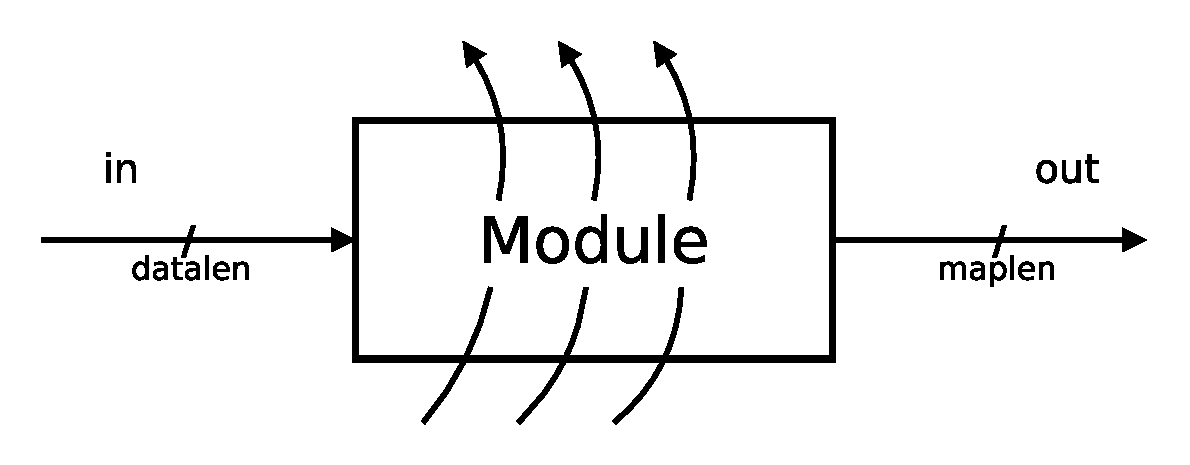
\epsfig{file=map.eps,width=0.8\columnwidth}%
\label{a}
\centering \caption{Digital Road Map}
\end{figure}
\clearpage
\subsection*{Motivation}
Generally GIS vector maps are extremely expensive to
produce. However, on the other hand, the digital nature 
of any vector map leaves it vulnerable to being copied 
and resold by a 3rd party without permission.


\myred{\bf Digital watermarking} is an important technique to protect the copyrights of digital products. 
\clearpage
A watermark is small amount of digital noise embedded into the digital representation of the products. 
\begin{figure}[h]
\centering
\subfigure[\scriptsize Note]{
  \label{fig:mqtree}
  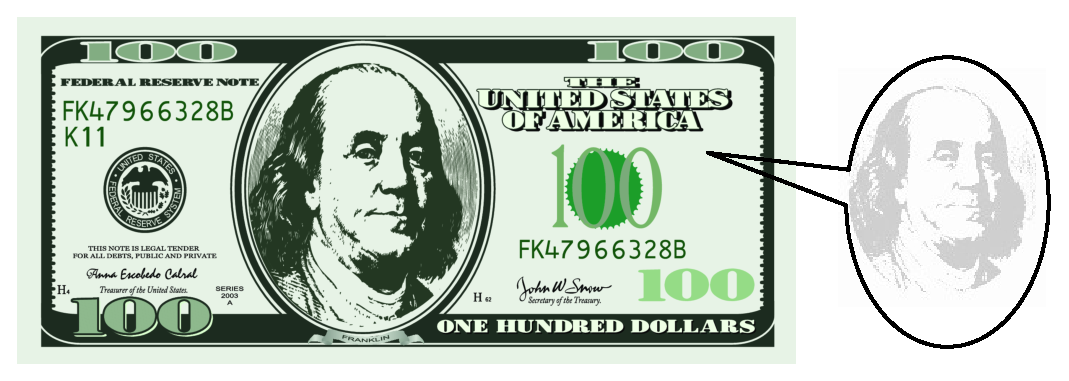
\epsfig{file=notemark.eps,width=0.55\columnwidth}
}
\subfigure[\scriptsize Digital map]{
  \label{fig:mqtree}
  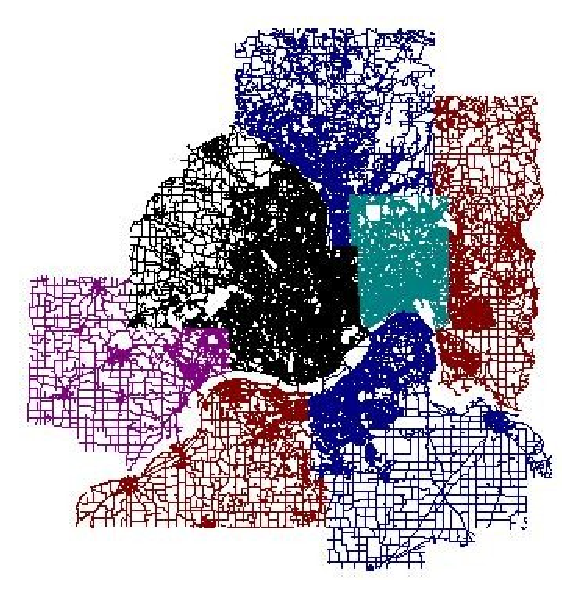
\epsfig{file=region.eps,width=0.25\columnwidth}
}
\caption{Watermark}
\label{fig:notemark}
\end{figure}
\clearpage

The standard watermarking framework for digital road maps 
 adopts a two-step approach -- the watermark \myred{\bf insertion} and \myred{\bf detection} algorithms.
\begin{figure}[h]
\centering
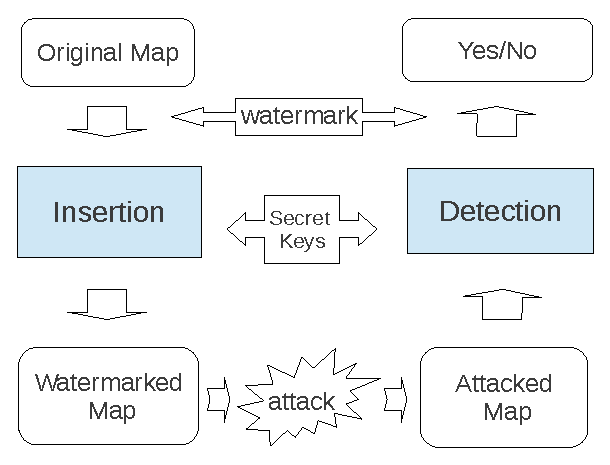
\epsfig{file=Flow.eps,width=0.4\columnwidth}
\caption{General Watermarking Framework For Road Maps}
\label{fig:workflow}
\end{figure}
\clearpage

%
% SLIDE 5 ----------------------------------------------------------
%
\section{Problem Definition}

\subsection*{Two specifical attacks}
\begin{enumerate}
	\item Noise attack
	\item Reorder attack
	\item Simplify/Addition attack
	\item \myred{Crop attack}
	\item \myred{Merge attack}
\end{enumerate}	
\clearpage
%
% SLIDE 6 ----------------------------------------------------------
%

\subsection*{Crop Attack}
An attacker crops a geographical region from the watermarked map
and use it as if it's a new map.
We define cropping attack as:
\[
Crop(M) = \{ subseg(R) ~|~ R \in M'\}
\]
where 
$M' \subseteq M$ and $subseq (R)$ returns a subsequence of road $R$.

\clearpage

\subsection*{Merge Attack}
An attacker crops parts from different maps and piece
them together to make a new map.
\begin{figure}[h]
\centering
\epsfig{file=overlap.eps,width=0.5\columnwidth}
\caption{Overlap of Two Maps}
\label{fig:17}
\end{figure}

\begin{figure}[h]
\centering
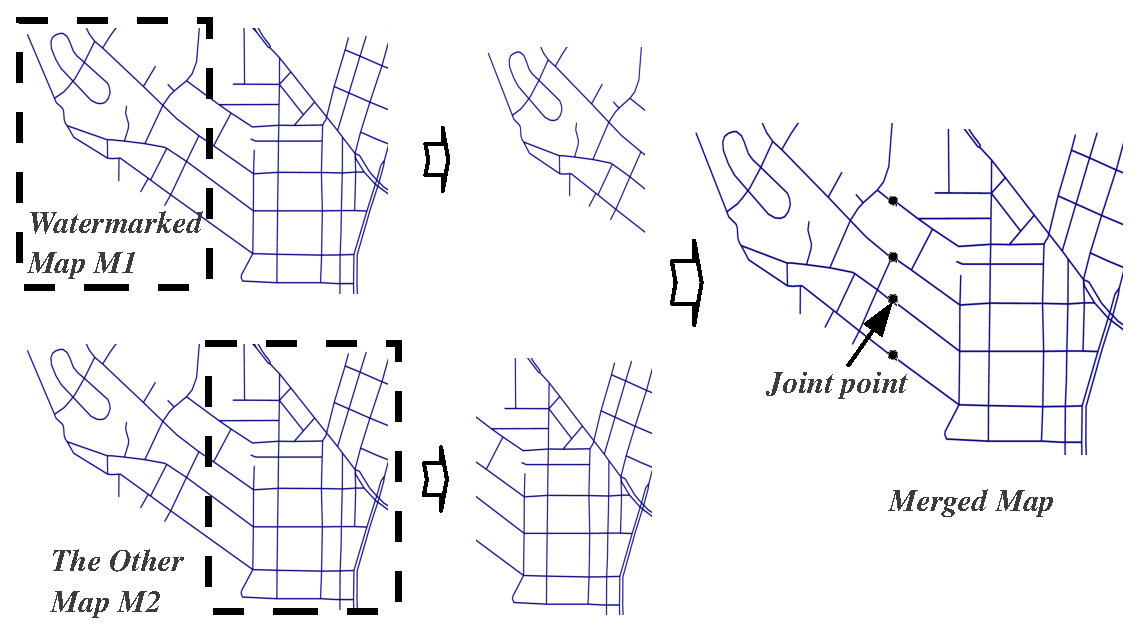
\epsfig{file=problem.eps, width=0.7\columnwidth}
\caption{Merge Attack}
\label{fig:merge}
\end{figure}

\clearpage
%
% SLIDE 7 ----------------------------------------------------------
%

%
% SLIDE 8 ----------------------------------------------------------
%
\section{Our approach}
\subsection*{Secret Keys}
 They should only be known to the map owner.
\subsubsection*{Secret Grid}
The {\bf secret grid} $G$ is a coordinate gird. 
\begin{itemize}
\item An origin, certain position with precise latitude and longitude
\item A step size, defines the granularity of the grid
\end{itemize}
\[G=\{Origin(x_0, y_0), Step\}\]
\clearpage
\subsubsection*{Secret MBR}
Given an original map to watermark, it can be laid out on the master grid, 
according to the coordinates of the vertices in the map. 
The {\bf secret MBR} is then the smallest
rectangle which coincides with the grid lines and completely 
encloses the whole map.
\clearpage

\begin{figure}[h]
\centering
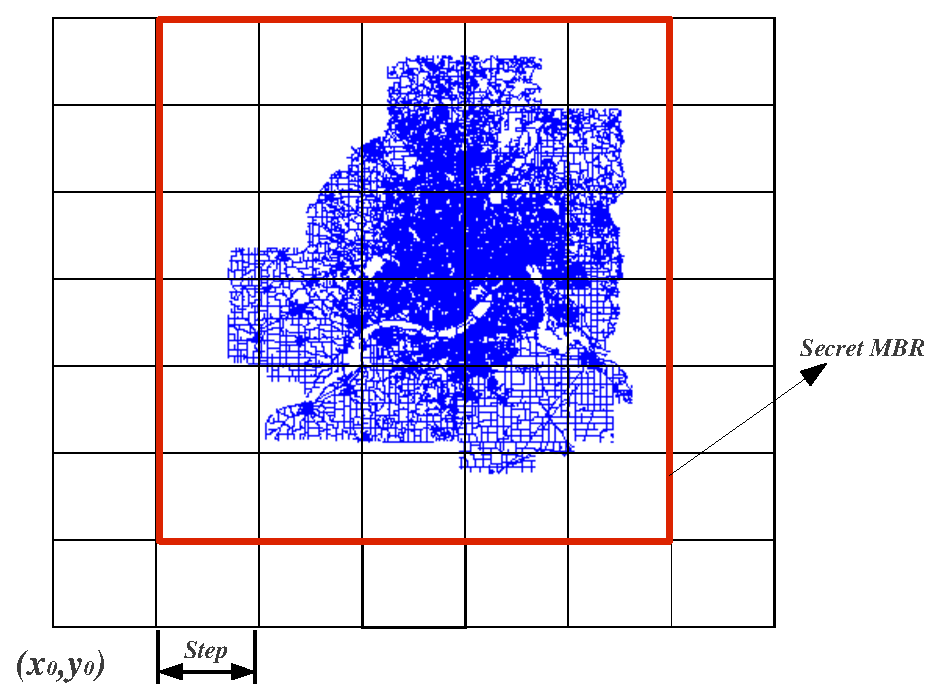
\epsfig{file=SecretGrid.eps,width=0.6\columnwidth}
\caption{Master Grid and MBR}
\label{fig:grid}
\end{figure}


\clearpage
\subsubsection*{Secret Square Size}
The {\bf secret square size} is an integer number $l$ that determines the size of a square box that we
used to select a small neighborhood of road segments from which to compute the watermarks.
\clearpage





\subsection*{Partition}
It recursively partitions the space bounded by the secret MBR for a map
into small regions using a modified quad-tree
structure (known as MQtree) according to the 
density of the roads. Each node in MQtree represents a sub-region of the map.
\begin{itemize}
\item if roads length within one region $> 4\theta$, partition it into 4 sub-regions.
\item if roads length within one region $< \theta$, merge it with neighbor.
\end{itemize}

\clearpage

\begin{figure}[th]
\centering
\subfigure[\scriptsize Map]{
  \label{fig:par}
  \epsfig{file=partition.eps,width=0.35\columnwidth}
}
\subfigure[\scriptsize MQtree]{
  \label{fig:mqtree}
  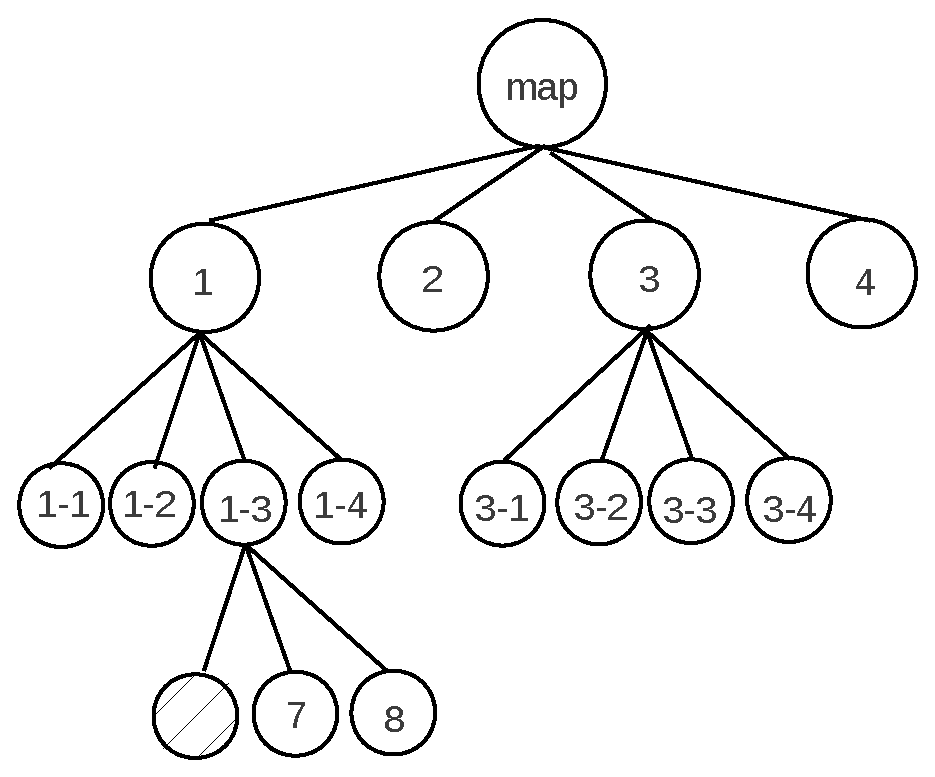
\epsfig{file=MQtree.eps,width=0.45\columnwidth}
}
\caption{MQtree}
\label{fig:quadtree}
\end{figure}
\clearpage
The time complexity of partition is 
\[\T = O(|E|\log\LEN),\]
where $\LEN$ is the total length of all roads in map $M$.
\clearpage

\subsection*{Insertion}
\begin{itemize}
\item The watermark is inserted into a road vertex $P(x, y)$ which is
closest to the center of the sub-region. 

\item The algorithm draws a square box of size $l$ centered at $P(x, y)$. 
\item Let $sl$ be the length of road segments that intersects the square box
\item Let $j$ be a value hashed from $sl$. 
\item Set the $j^{th}$ least significant bit in $x$ coordinate of $P$ to ``1''. 
\end{itemize}
\clearpage

\begin{figure}
\centering
\epsfig{file=insertion.eps,width=0.4\columnwidth}
\label{fig:insert}
\caption{Insertion Strategy}
\end{figure} 
\clearpage

The hash function in this algorithm must 
guarantee to hash to the same value before and after watermarking. 
Even if the watermarked map is attacked, the hash function must still hash to the same $j$. 

$J_{max}$: the biggest LSB that can be changed within the possible distortion of a single end point.
\begin{eqnarray*}
j&=&Hash(Trans(sl),k) \\
&\rm{where} & Trans(x)= x \land \underbrace {11\ldots1\overbrace {00\ldots0}^{J_{max}} }_{bit\_length(x)} 
\end{eqnarray*}
\clearpage




\subsection*{Detection}
We partition the map using the same strategy as insertion. Then we select the data points closest
to the center of the regions to detect whether the watermark exists there.

Each sub-region which is detected to contain a watermark casts a vote
which collectively contributes to the final decision of whether a larger
area is watermarked as a whole.

\clearpage

\begin{figure}[h]
\centering
\subfigure[\scriptsize Map]{
  \label{fig:parcrop}
  \epsfig{file=parcrop.eps,width=0.35\columnwidth}
}
\subfigure[\scriptsize MQtree]{
  \label{fig:mqtreecrop}
  \epsfig{file=MQtreecrop.eps,width=0.45\columnwidth}
}
\caption{Detection Strategy}
\label{fig:detect}
\end{figure} 
\clearpage

\subsection*{Confidence}
We define the detection confidence of detection as
\begin{equation} \label{eqn:conf}
conf=1 - \sum _{ i=n }^N{N \choose i}\left(\frac{1}{2}\right)^{ N-i} 
\left(\frac{1}{2}\right)^i 
\end{equation}
where $N$ is total number of leaf nodes and $n$ is number of leaf nodes that match. 
\clearpage


\mybox{0.8\textwidth}{%
  \begin{theorem}[Detection Confidence]\label{murphy}
    Given a map $M$ with total length $\LEN$ and an algorithm threshold $\theta$, 
the minimum detection confidence for $M$: 
\[
\label{pe}
conf_{min}(M) = 1 - \sum _{ i={\lceil\rho\LEN/{4 \theta}\rceil} }^{ \lceil\LEN/{4 \theta}\rceil}
{{\lceil \LEN/{4 \theta}\rceil \choose i} {\left(\frac{1}{2}\right)}^{\lceil \LEN/{4 \theta}\rceil}} 
\]
where $\rho$ is the ratio between the number of leaf nodes that match and
the total number of leaf nodes in $M$. 
  \end{theorem}
} 
%\begin{proof}
%  A special case of Theorem \ref{murphy} is proven in the textbook.
%\end{proof}
\clearpage
\begin{figure}[h]
\centering
\epsfig{file=security.eps,width=0.7\columnwidth}
\caption{Accuracy of Detection}
\label{fig:security}
\end{figure} 
\clearpage
%
% SLIDE 9 ----------------------------------------------------------
%
\section{Experiment Results}
We implement and test the performance of the algorithms 
under different potential attacks. The map data is from two different sources, MN/DOT\cite{mndoturl} and United States Census Website\cite{tigerurl}.

We compare the proposed approach with two other 
watermarking algorithms proposed by Pu\cite{PuDJ06} and 
Voigt\cite{Voigt:2003}. Both methods are blind watermarking algorithms and provide some resistance to crop attack.
\clearpage
\subsection*{Performance under Cropping}
The partition criterion $\theta $ has a large influence on the result of our watermark algorithm. We also design a series of experiments to figure out the influence of the $\theta $. 
\clearpage

\begin{table}[h]
\centering
\label{tab:crop}
\begin{tabular}{|c||c|c|c|c|} 
\hline
County & Total & Match & Confidence & Result \\\hline \hline
Anoka & 55 & 51 & 1.000 & positive\\\hline
Carver & 28 & 23 & 0.999 & positive\\\hline
Dakota & 68 & 61 & 1.000 & positive\\\hline
Hennipin & 141 & 137 & 1.000 & positive\\\hline
Ramsey & 58 & 56 & 1.000 & positive\\\hline
Scott & 29 & 25 & 0.999 & positive\\\hline
Washington & 46 & 43 & 1.000 & positive\\\hline
\end{tabular}
\caption{Crop Attack Detection}
\end{table}
\clearpage

%In this experiment, we watermark the map with different distortion by adjusting $\theta $  and then select the crop ratio of $1/2$, $1/4$ and $1/8$ of the map to detect. Each ratio is detected for 20 times.
\clearpage

\begin{figure}[h]
\centering
\subfigure[Distortion]{
  \label{fig:dis}
  \epsfig{file=mdelta.eps,width=0.3\columnwidth}
}
\subfigure[Different Crop Ratio]{
  \label{fig:m}
  \epsfig{file=mparameter.eps,width=0.3\columnwidth}
}\\
\subfigure[Time of Insertion]{
  \label{fig:ti}
  \epsfig{file=time.eps,width=0.3\columnwidth}
}
\subfigure[Time of Detection]{
  \label{fig:td}
  \epsfig{file=time1.eps,width=0.3\columnwidth}
}
\label{fig:pudd}
\end{figure}

\clearpage

\begin{figure}[h]
\centering
\subfigure[\scriptsize Performance under Cropping]{
  \label{fig:cropattack}
  \epsfig{file=cropattack.eps,width=0.4\columnwidth}
}
\subfigure[\scriptsize Accuracy in $1/8$ crop ratio]{
  \label{fig:mdelta}
  \epsfig{file=delta.eps,width=0.4\columnwidth}
}
\caption{Performance under Crop Attack}
\end{figure}
\clearpage


\subsection*{Performance under merging}
\begin{figure}[h]
\centering
\label{fig:mattack}
\epsfig{file=mattack.eps,width=0.3\columnwidth}
\caption{Merge Attack}
\end{figure}
\clearpage
\subsubsection*{Detection Result}
\begin{table}[th]
\centering
\label{tab:merge}
\begin{tabular}{|c||c|c|c|c|} 
\hline
Region & Total & Match & Confidence & Result \\\hline \hline
1 & 147 & 122 & 1.000 & positive\\\hline
2 & 12 & 11 & 0.997 & positive\\\hline
3 & 23 & 18 & 0.994 & positive\\\hline
4 & 15 & 12 & 0.983 & positive\\\hline
\end{tabular}
\caption{Merge Attack Detection}
\end{table}
\clearpage


\begin{figure}[h]
\centering
\label{fig:mresult}
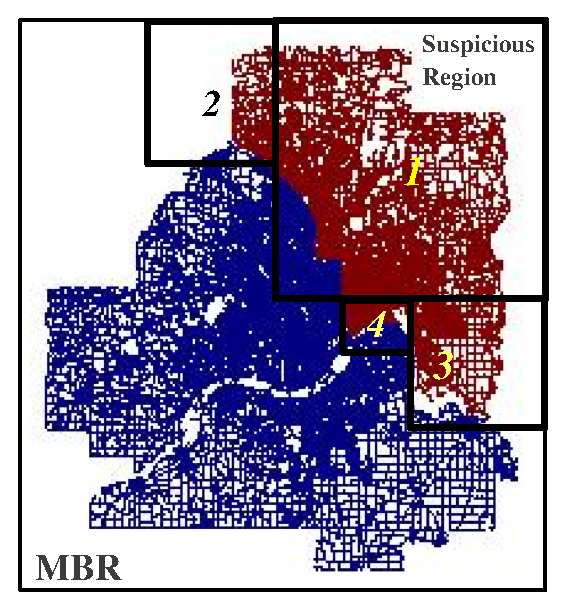
\epsfig{file=mresult.eps,width=0.4\columnwidth}
\caption{Merged Map}
\end{figure}
\clearpage

\begin{figure}[h]
\centering
\subfigure[\scriptsize Performance under merging]{
  \label{fig:mergeattack}
  \epsfig{file=mergeattack.eps,width=0.47\columnwidth}
}
\subfigure[\scriptsize Accuracy in $1/8$ merge ratio]{
  \label{fig:deltamerge}
  \epsfig{file=deltamerge.eps,width=0.47\columnwidth}
}
\caption{Performance under Merge Attack}
\end{figure}

\clearpage
\section{Conclusion}
\begin{enumerate}
		\item We proposed a new blind watermarking scheme for digital vector road maps. 
\item The algorithm dynamically partitions a given map according to
road density and inserts one-bit watermarks to one of the least significant bits
of points. 
\item Our preliminary evaluation shows that this algorithm 
is resilient to massive crop and merge attacks.
\end{enumerate}
\clearpage

%------------------------------------------------

\thispagestyle{empty} % No slide header and footer

\bibliographystyle{unsrt}
\bibliography{watermark}

\clearpage
%
% SLIDE  ----------------------------------------------------------
%
\thispagestyle{empty}
% background (stroke)
\begin{tikzpicture}[remember picture,overlay]
	\node [xshift=\paperwidth/2,yshift=\paperheight/2] at (current page.south west)[rectangle,fill,inner sep=0pt,minimum width=\paperwidth,minimum height=\paperheight/3,top color=mygreen,bottom color=mygreen]{};
\end{tikzpicture}%
% content
\begin{flushright}
	\vspace{0.6cm}
	\color{white}\sffamily
	{\bfseries\Large
	Questions?	
	\par}
	\vfill
%	\includegraphics[width=0.25\textwidth]{./contents/logo}%
\end{flushright}
% ------------------------------------------------------------------------------
% End document
% ------------------------------------------------------------------------------
\end{document}
